
%% \documentclass[]{report}
\documentclass[preprint,10pt]{sigplanconf}
% The following \documentclass options may be useful:

% preprint      Remove this option only once the paper is in final form.
% 10pt          To set in 10-point type instead of 9-point.
% 11pt          To set in 11-point type instead of 9-point.
% authoryear    To obtain author/year citation style instead of numeric.

% \usepackage[a4paper]{geometry}
\usepackage[dvips]{graphicx}            % to include images
%\usepackage{pslatex}	    % to use PostScript fonts

\begin{document}

%%\special{papersize=8.5in,11in}
%%\setlength{\pdfpageheight}{\paperheight}
%%\setlength{\pdfpagewidth}{\paperwidth}

\conferenceinfo{}{} 
\copyrightyear{2014} 
\copyrightdata{978-1-nnnn-nnnn-n/yy/mm} 
\doi{nnnnnnn.nnnnnnn}

\titlebanner{Draft \#0, April 2014}
\preprintfooter{Draft \#0, April 2014}

\title{Chain Replication metadata management in Machi, an immutable
  file store}
\subtitle{Introducing the ``humming consensus'' algorithm}

\authorinfo{Basho Japan KK}{}

\maketitle

\section{Origins}
\label{sec:origins}

This document was first written during the autumn of 2014 for a
Basho-only internal audience.  Since its original drafts, Machi has
been designated by Basho as a full open source software project.  This
document has been rewritten in 2015 to address an external audience.
For an overview of the design of the larger Machi system, please see
\cite{machi-design}.

\section{Abstract}
\label{sec:abstract}

TODO Fix, after all of the recent changes to this document.

Machi is an immutable file store, now in active development by Basho
Japan KK.  Machi uses Chain Replication to maintain strong consistency
of file updates to all replica servers in a Machi cluster.  Chain
Replication is a variation of primary/backup replication where the
order of updates between the primary server and each of the backup
servers is strictly ordered into a single ``chain''.  Management of
Chain Replication's metadata, e.g., ``What is the current order of
servers in the chain?'', remains an open research problem.  The
current state of the art for Chain Replication metadata management
relies on an external oracle (e.g., ZooKeeper) or the Elastic
Replication algorithm.

This document describes the Machi chain manager, the component
responsible for managing Chain Replication metadata state.  The chain
manager uses a new technique, based on a variation of CORFU, called
``humming consensus''.

Humming consensus does not require active participation by all or even
a majority of participants to make decisions.  Machi's chain manager
bases its logic on humming consensus to make decisions about how to
react to changes in its environment, e.g. server crashes, network
partitions, and changes by Machi cluster admnistrators.  Once a
decision is made during a virtual time epoch, humming consensus will
eventually discover if other participants have made a different
decision during that epoch.  When a differing decision is discovered,
new time epochs are proposed in which a new consensus is reached and
disseminated to all available participants.

\section{Introduction}
\label{sec:introduction}

\subsection{What does ``self-management'' mean?}
\label{sub:self-management}

For the purposes of this document, chain replication self-management
is the ability for the $N$ nodes in an $N$-length chain replication chain
to manage the chain's metadata without requiring an external party
to perform these management tasks.  Chain metadata state and state
management tasks include:

\begin{itemize}
\item Preserving data integrity of all metadata and data stored within
  the chain.  Data loss is not an option.
\item Stably preserve knowledge of chain membership (i.e. all nodes in
   the chain, regardless of operational status). A systems
   administrators is expected to make ``permanent'' decisions about
   chain membership.
\item Using passive and/or active techniques to track operational
   state/status, e.g., up, down, restarting, full data sync, partial
   data sync, etc.
\item Choosing the run-time replica ordering/state of the chain, based on
   current member status and past operational history.  All chain
   state transitions must be done safely and without data loss or
   corruption.
\item As a new node is added to the chain administratively or old node is
   restarted, adding the node to the chain safely and perform any data
   synchronization/repair required to bring the node's data into
   full synchronization with the other nodes.
\end{itemize}

\subsection{Ultimate goal: Preserve data integrity of Chain Replicated data}

Preservation of data integrity is paramount to any chain state
management technique for Machi.  Even when operating in an eventually
consistent mode, Machi must not lose data without cause outside of all
design, e.g., all particpants crash permanently.

\subsection{Goal: Contribute to Chain Replication metadata management research}

We believe that this new self-management algorithm, humming consensus,
contributes a novel approach to Chain Replication metadata management.
Typical practice in the IT industry appears to favor using an external
oracle, e.g., using ZooKeeper as a trusted coordinator.  The ``monitor
and mangage your neighbor'' technique proposed in elastic replication
(Section \ref{ssec:elastic-replication}) appears to be the current
state of the art in the distributed systems research community.

See Section~\ref{sec:cr-management-review} for a brief review.

\subsection{Goal: Support both eventually consistent \& strongly consistent modes of operation}

Machi's first use cases are all for use as a file store in an eventually
consistent environment.
Later, we wish the option of supporting strong consistency
applications such as CORFU-style logging while reusing all (or most)
of Machi's infrastructure.

In eventually consistent mode, humming consensus
allows a Machi cluster to fragment into
arbitrary islands of network partition, all the way down to 100\% of
members running in complete network isolation from each other.
Furthermore, it provides enough agreement to allow
formerly-partitioned members to coordinate the reintegration and
reconciliation of their data when partitions are healed.

\subsection{Anti-goal: Minimize churn}

Humming consensus's goal is to manage Chain Replication metadata
safely.  If participants have differing notions of time, e.g., running
on extremely fast or extremely slow hardware, then humming consensus
may "churn" rapidly in different metadata states in such a way that
the chain's data would be effectively unavailable.  

In practice, however, any series of network partition changes that
case humming consensus to churn will cause other management techniques
(such as an external "oracle") similar problems.
{\bf [Proof by handwaving assertion.]}
(See also: Section~\ref{sub:time-model})

\section{Review of current Chain Replication metadata management methods}
\label{sec:cr-management-review}

We briefly survey the state of the art of research and industry
practice of chain replication metadata management options.

\subsection{``Leveraging Sharding in the Design of Scalable Replication Protocols'' by Abu-Libdeh, van Renesse, and Vigfusson}
\label{ssec:elastic-replication}
Multiple chains are arranged in a ring (called a "band" in the paper).
The responsibility for managing the chain at position N is delegated
to chain N-1.  As long as at least one chain is running, that is
sufficient to start/bootstrap the next chain, and so on until all
chains are running.  This technique is called ``Elastic Replication''.

The paper then estimates mean-time-to-failure
(MTTF) and suggests a "band of bands" topology to handle very large
clusters while maintaining an MTTF that is as good or better than
other management techniques.

{\bf NOTE:} If the chain self-management method proposed for Machi does not
succeed, this paper's technique is our best fallback recommendation.

\subsection{An external management oracle, implemented by ZooKeeper}
\label{ssec:an-oracle}
This is not a recommendation for Machi: we wish to avoid using
ZooKeeper and any other ``large'' external service dependency.  See
the ``Assumptions'' section of \cite{machi-design} for Machi's overall
design assumptions and limitations.

However, many other open source software products use ZooKeeper for
exactly this kind of critical metadata replica management problem.

\subsection{An external management oracle, implemented by Riak Ensemble}

This is a much more palatable choice than option~\ref{ssec:an-oracle}
above.  We also
wish to avoid an external dependency on something as big as Riak
Ensemble.  However, if it comes between choosing Riak Ensemble or
choosing ZooKeeper, the choice feels quite clear: Riak Ensemble will
win, unless there is some critical feature missing from Riak
Ensemble.  If such an unforseen missing feature is discovered, it
would probably be preferable to add the feature to Riak Ensemble
rather than to use ZooKeeper (and for Basho to document ZK, package
ZK, provide commercial ZK support, etc.).

\section{Assumptions}
\label{sec:assumptions}

Given a long history of consensus algorithms (viewstamped replication,
Paxos, Raft, et al.), why bother with a slightly different set of
assumptions and a slightly different protocol?

The answer lies in one of our explicit goals: to have an option of
running in an "eventually consistent" manner.  We wish to be able to
make progress, i.e., remain available in the CAP sense, even if we are
partitioned down to a single isolated node.  VR, Paxos, and Raft
alone are not sufficient to coordinate service availability at such
small scale.  The humming consensus algorithm can manage
both strongly consistency systems (i.e., the typical use for Chain
Replication) as well as eventually consistent data systems.

\subsection{The CORFU protocol is correct}

This work relies tremendously on the correctness of the CORFU
protocol \cite{corfu1}, a cousin of the Paxos protocol.
If the implementation of
this self-management protocol breaks an assumption or prerequisite of
CORFU, then we expect that Machi's implementation will be flawed.

\subsection{Communication model}

The communication model is asynchronous point-to-point messaging.
The network is unreliable: messages may be arbitrarily dropped and/or
reordered.  Network partitions may occur at any time.
Network partitions may be asymmetric, e.g., a message can be sent successfully
from $A \rightarrow B$, but messages from $B \rightarrow A$ can be
lost, dropped, and/or arbitrarily delayed.

System particpants may be buggy but not actively malicious/Byzantine.

\subsection{Time model}
\label{sub:time-model}

Our time model is per-node wall-clock time clocks, loosely
synchronized by NTP.

The protocol and algorithm presented here do not specify or require any
timestamps, physical or logical.  Any mention of time inside of data
structures are for human/historic/diagnostic purposes only.

Having said that, some notion of physical time is suggested for
purposes of efficiency.  It's recommended that there be some "sleep
time" between iterations of the algorithm: there is no need to "busy
wait" by executing the algorithm as quickly as possible.  See below,
"sleep intervals between executions".

\subsection{Failure detector model}

We assume that the failure detector that the algorithm uses is weak,
it's fallible, and it informs the algorithm in boolean status
updates/toggles as a node becomes available or not.

If the failure detector is fallible and tells us a mistaken status
change, then the algorithm will "churn" the operational state of the
chain, e.g. by removing the failed node from the chain or adding a
(re)started node (that may not be alive) to the end of the chain.
Such extra churn is regrettable and will cause periods of delay as the
humming consensus algorithm (decribed below) makes decisions.  However, the
churn cannot {\bf (we assert/believe)} cause data loss.

\subsection{Data consistency: strong unless otherwise noted}

Most discussion in this document assumes a desire to preserve strong
consistency in all data managed by Machi's chain replication.  We
use the short-hand notation ``CP mode'' to describe this default mode
of operation, where ``C'' and ``P'' refer to the CAP Theorem
\cite{cap-theorem}.

However, there are interesting use cases where Machi is useful in a
more relaxed, eventual consistency environment.  We may use the
short-hand ``AP mode'' when describing features that preserve only
eventual consistency.  Discussion of AP mode features in this document
will always be explictly noted --- discussion of strongly consistent CP
mode is always the default.

\subsection{Use of the ``wedge state''}

A participant in Chain Replication will enter "wedge state", as
described by the Machi high level design \cite{machi-design} and by CORFU,
when it receives information that
a newer projection (i.e., run-time chain state reconfiguration) is
available.  The new projection may be created by a system
administrator or calculated by the self-management algorithm.
Notification may arrive via the projection store API or via the file
I/O API.

When in wedge state, the server will refuse all file write I/O API
requests until the self-management algorithm has determined that
humming consensus has been decided (see next bullet item).  The server
may also refuse file read I/O API requests, depending on its CP/AP
operation mode.

\subsection{Use of ``humming consensus''}

CS literature uses the word "consensus" in the context of the problem
description at \cite{wikipedia-consensus}
.
This traditional definition differs from what is described here as
``humming consensus''.

"Humming consensus" describes
consensus that is derived only from data that is visible/known at the current
time.
The algorithm will calculate
a rough consensus despite not having input from all/majority
of chain members.  Humming consensus may proceed to make a
decision based on data from only a single participant, i.e., only the local
node.

See Section~\ref{sec:humming-consensus} for detailed discussion.

\subsection{Concurrent chain managers execute humming consensus independently}

Each Machi file server has its own concurrent chain manager
process(es) embedded within it.  Each chain manager process will
execute the humming consensus algorithm using only local state (e.g.,
the $P_{current}$ projection currently used by the local server) and
values written and read from everyone's projection stores.

The chain manager's primary communication method with the local Machi
file API server is the wedge and un-wedge request API.  When humming
consensus has chosen a projection $P_{new}$ to replace $P_{current}$,
the value of $P_{new}$ is included in the un-wedge request.

\section{The projection store}

The Machi chain manager relies heavily on a key-value store of
write-once registers called the ``projection store''.
Each Machi node maintains its own projection store.
The store's keyspace is divided into two halves (described below),
each with different rules for who can write keys to that half of the
store.

The store's key is a 2-tuple of a positive integer and the half of
the partition, the ``public'' half or the ``private'' half.
The integer represents the epoch number of the projection stored with
this key.  The
store's value is either the special `unwritten' value\footnote{We use
  $\bot$ to denote the unwritten value.} or else a binary blob that is
immutable thereafter; the projection data structure is
serialized and stored in this binary blob.

The projection store is vital for the correct implementation of humming
consensus (Section~\ref{sec:humming-consensus}).  The write-once
register primitive allows us to analyze the store's behavior
using the same logical tools and techniques as the CORFU log.

\subsection{The publicly-writable half of the projection store}

The publicly-writable projection store is used to share information
during the first half of humming consensus algorithm.  Projections
in the public half of the store form a log of
suggestions\footnote{I hesitate to use the word ``propose'' or ``proposal''
  anywhere in this document \ldots until I've done a more formal
  analysis of the protocol.  Those words have too many connotations in
  the context of consensus protocols such as Paxos and Raft.}
by humming consensus participants for how they wish to change the
chain's metadata state.

Any chain member may write to the public half of the store.
Any chain member may read from the public half of the store.

\subsection{The privately-writable half of the projection store}

The privately-writable projection store is used to store the
Chain Replication metadata state (as chosen by humming consensus)
that is in use now (or has been used in the past) by the local Machi server.

Only the local server may write values into the private half of store.
Any chain member may read from the private half of the store.

The private projection store serves multiple purposes, including:

\begin{itemize}
\item Remove/clear the local server from ``wedge state''.
\item Act as a publicly-readable indicator of what projection that the
  local server is currently using.  This special projection will be
  called $P_{current}$ throughout this document.
\item Act as the local server's log/history of
  its sequence of $P_{current}$ projection changes.
\end{itemize}

The private half of the projection store is not replicated.

Projections in the private projection store are
meaningful only to the local Machi server and, furthermore, are
merely ``soft state''.  Data loss in the private projection store
cannot result in loss of ``hard state'' information.  Therefore,
replication of the private projection store is not required.  The
replication techniques described by
Section~\ref{sec:managing-multiple-projection-stores} applies only to
the public half of the projection store.

\section{Projections: calculation, storage, and use}
\label{sec:projections}

Machi uses a ``projection'' to determine how its Chain Replication replicas
should operate; see \cite{machi-design} and
\cite{corfu1}.  At runtime, a cluster must be able to respond both to
administrative changes (e.g., substituting a failed server box with
replacement hardware) as well as local network conditions (e.g., is
there a network partition?).

The projection defines the operational state of Chain Replication's
chain order as well the (re-)synchronization of data managed by by
newly-added/failed-and-now-recovering members of the chain.  This
chain metadata, together with computational processes that manage the
chain, must be managed in a safe manner in order to avoid unintended
data loss of data managed by the chain.

The concept of a projection is borrowed
from CORFU but has a longer history, e.g., the Hibari key-value store
\cite{cr-theory-and-practice} and goes back in research for decades,
e.g., Porcupine \cite{porcupine}.

\subsection{The projection data structure}
\label{sub:the-projection}

{\bf NOTE:} This section is a duplicate of the ``The Projection and
the Projection Epoch Number'' section of \cite{machi-design}.

The projection data
structure defines the current administration \& operational/runtime
configuration of a Machi cluster's single Chain Replication chain.
Each projection is identified by a strictly increasing counter called
the Epoch Projection Number (or more simply ``the epoch'').

Projections are calculated by each server using input from local
measurement data, calculations by the server's chain manager
(see below), and input from the administration API.
Each time that the configuration changes (automatically or by
administrator's request), a new epoch number is assigned
to the entire configuration data structure and is distributed to
all servers via the server's administration API.  Each server maintains the
current projection epoch number as part of its soft state.

Pseudo-code for the projection's definition is shown in
Figure~\ref{fig:projection}.  To summarize the major components:

\begin{figure}
\begin{verbatim}
-type m_server_info() :: {Hostname, Port,...}.
-record(projection, {
            epoch_number    :: m_epoch_n(),
            epoch_csum      :: m_csum(),
            creation_time   :: now(),
            author_server   :: m_server(),
            all_members     :: [m_server()],
            active_upi      :: [m_server()],
            active_all      :: [m_server()],
            down_members    :: [m_server()],
            dbg_annotations :: proplist()
        }).
\end{verbatim}
\caption{Sketch of the projection data structure}
\label{fig:projection}
\end{figure}

\begin{itemize}
\item {\tt epoch\_number} and {\tt epoch\_csum} The epoch number and
  projection checksum are unique identifiers for this projection.
\item {\tt creation\_time} Wall-clock time, useful for humans and
  general debugging effort.
\item {\tt author\_server} Name of the server that calculated the projection.
\item {\tt all\_members} All servers in the chain, regardless of current
  operation status.  If all operating conditions are perfect, the
  chain should operate in the order specified here.
\item {\tt active\_upi} All active chain members that we know are
  fully repaired/in-sync with each other and therefore the Update
  Propagation Invariant (Section~\ref{sub:upi} is always true.
\item {\tt active\_all} All active chain members, including those that
  are under active repair procedures.
\item {\tt down\_members} All members that the {\tt author\_server}
  believes are currently down or partitioned.
\item {\tt dbg\_annotations} A ``kitchen sink'' proplist, for code to
  add any hints for why the projection change was made, delay/retry
  information, etc.
\end{itemize}

\subsection{Why the checksum field?}

According to the CORFU research papers, if a server node $S$ or client
node $C$ believes that epoch $E$ is the latest epoch, then any information
that $S$ or $C$ receives from any source that an epoch $E+\delta$ (where
$\delta > 0$) exists will push $S$ into the "wedge" state and $C$ into a mode
of searching for the projection definition for the newest epoch.

In the humming consensus description in
Section~\ref{sec:humming-consensus}, it should become clear that it's
possible to have a situation where two nodes make proposals
for a single epoch number.  In the simplest case, assume a chain of
nodes $A$ and $B$.  Assume that a symmetric network partition between
$A$ and $B$ happens. Also, let's assume that operating in
AP/eventually consistent mode.

On $A$'s network-partitioned island, $A$ can choose
an active chain definition of {\tt [A]}.
Similarly $B$ can choose a definition of {\tt [B]}.  Both $A$ and $B$
might choose the
epoch for their proposal to be \#42.  Because each are separated by
network partition, neither can realize the conflict.

When the network partition heals, it can become obvious to both
servers that there are conflicting values for epoch \#42.  If we
use CORFU's protocol design, which identifies the epoch identifier as
an integer only, then the integer 42 alone is not sufficient to
discern the differences between the two projections.

Humming consensus requires that any projection be identified by both
the epoch number and the projection checksum, as described in
Section~\ref{sub:the-projection}.

\section{Managing multiple projection store replicas}
\label{sec:managing-multiple-projection-stores}

An independent replica management technique very similar to the style
used by both Riak Core \cite{riak-core} and Dynamo is used to manage
replicas of Machi's projection data structures.
The major difference is that humming consensus
{\em does not necessarily require}
successful return status from a minimum number of participants (e.g.,
a quorum).

\subsection{Read repair: repair only unwritten values}

The idea of ``read repair'' is also shared with Riak Core and Dynamo
systems.  However, Machi has situations where read repair cannot truly
``fix'' a key because two different values have been written by two
different replicas.
Machi's projection store is write-once, and there is no ``undo'' or
``delete'' or ``overwrite'' in the projection store API.\footnote{It doesn't
matter what caused the two different values.  In case of multiple
values, all participants in humming consensus merely agree that there
were multiple suggestions at that epoch which must be resolved by the
creation and writing of newer projections with later epoch numbers.}
Machi's projection store read repair can only repair values that are
unwritten, i.e., storing $\bot$.

The value used to repair $\bot$ values is the ``best'' projection that
is currently available for the current epoch $E$.  If there is a single,
unanimous value $V_{u}$ for the projection at epoch $E$, then $V_{u}$
is use to repair all projections stores at $E$ that contain $\bot$
values.  If the value of $K$ is not unanimous, then the ``highest
ranked value'' $V_{best}$ is used for the repair; see
Section~\ref{sub:ranking-projections} for a description of projection
ranking.

\subsection{Writing to public projection stores}
\label{sub:proj-store-writing}

Writing replicas of a projection $P_{new}$ to the cluster's public
projection stores is similar, in principle, to writing a Chain
Replication-managed system or Dynamo-like system.  But unlike Chain
Replication, the order doesn't really matter.
In fact, the two steps below may be performed in parallel.
The significant difference with Chain Replication is how we interpret
the return status of each write operation.

\begin{enumerate}
\item Write $P_{new}$ to the local server's public projection store
  using $P_{new}$'s epoch number $E$ as the key.
  As a side effect, a successful write will trigger
  ``wedge'' status in the local server, which will then cascade to other
  projection-related activity by the local chain manager.
\item Write $P_{new}$ to key $E$ of each remote public projection store of
  all participants in the chain.
\end{enumerate}

In cases of {\tt error\_written} status,
the process may be aborted and read repair
triggered.  The most common reason for {\tt error\_written} status
is that another actor in the system has
already calculated another (perhaps different) projection using the
same projection epoch number and that
read repair is necessary.  The {\tt error\_written} may also
indicate that another server has performed read repair on the exact
projection $P_{new}$ that the local server is trying to write!

\subsection{Writing to private projection stores}

Only the local server/owner may write to the private half of a
projection store.  Also, the private projection store is not replicated.

\subsection{Reading from public projection stores}
\label{sub:proj-store-reading}

A read is simple: for an epoch $E$, send a public projection read API
request to all participants.  As when writing to the public projection
stores, we can ignore any timeout/unavailable return
status.\footnote{The success/failure status of projection reads and
  writes is {\em not} ignored with respect to the chain manager's
  internal liveness tracker.  However, the liveness tracker's state is
  typically only used when calculating new projections.}  If we
discover any unwritten values $\bot$, the read repair protocol is
followed.

The minimum number of non-error responses is only one.\footnote{The local
projection store should always be available, even if no other remote
replica projection stores are available.}  If all available servers
return a single, unanimous value $V_u, V_u \ne \bot$, then $V_u$ is
the final result for epoch $E$.
Any non-unanimous values are considered complete disagreement for the
epoch.  This disagreement is resolved by humming consensus by later
writes to the public projection stores during subsequent iterations of
humming consensus.

We are not concerned with unavailable servers.  Humming consensus
only uses as many public projections as are available at the present
moment of time.  If some server $S$ is unavailable at time $t$ and
becomes available at some later $t+\delta$, and if at $t+\delta$ we
discover that $S$'s public projection store for key $E$
contains some disagreeing value $V_{weird}$, then the disagreement
will be resolved in the exact same manner that would be used as if we
had found the disagreeing values at the earlier time $t$ (see previous
paragraph).

\section{Phases of projection change, a prelude to Humming Consensus}
\label{sec:phases-of-projection-change}

Machi's use of projections is in four discrete phases and are
discussed below: network monitoring,
projection calculation, projection storage, and
adoption of new projections.  The phases are described in the
subsections below.  The reader should then be able to recognize each
of these phases when reading the humming consensus algorithm
description in Section~\ref{sec:humming-consensus}.

TODO should this section simply (?) be merged with Section~\ref{sec:humming-consensus}?

\subsection{Network monitoring}
\label{sub:network-monitoring}

Monitoring of local network conditions can be implemented in many
ways.  None are mandatory, as far as this RFC is concerned.
Easy-to-maintain code should be the primary driver for any
implementation.  Early versions of Machi may use some/all of the
following techniques:

\begin{itemize}
\item Internal ``no op'' FLU-level protocol request \& response.
\item Explicit connections of remote {\tt epmd} services, e.g., to
tell the difference between a dead Erlang VM and a dead
machine/hardware node.
\item Network tests via ICMP {\tt ECHO\_REQUEST}, a.k.a. {\tt ping(8)}
\end{itemize}

Output of the monitor should declare the up/down (or
alive/unknown) status of each server in the projection.  Such
Boolean status does not eliminate fuzzy logic, probabilistic
methods, or other techniques for determining availability status.
A hard choice of boolean up/down status
is required only by the projection calculation phase
(Section~\ref{sub:projection-calculation}).

\subsection{Calculating a new projection data structure}
\label{sub:projection-calculation}

A new projection may be
required whenever an administrative change is requested or in response
to network conditions (e.g., network partitions, crashed server).

Projection calculation is a pure computation, based on input of:

\begin{enumerate}
\item The current projection epoch's data structure
\item Administrative request (if any)
\item Status of each server, as determined by network monitoring
(Section~\ref{sub:network-monitoring}).
\end{enumerate}

Decisions about {\em when} to calculate a projection are made
using additional runtime information.  Administrative change requests
probably should happen immediately.  Change based on network status
changes may require retry logic and delay/sleep time intervals.

\subsection{Writing a new projection}
\label{sub:proj-storage-writing}

Let's ignore humming consensus for a moment and consider the general
case for Chain Replication and strong consistency.  Any manager of
chain state metadata must maintain a history of the current chain
state and some history of prior states.  Strong consistency can be
violated if this history is forgotten.

In Machi's case, the writing a new projection phase is very
straightforward; see
Section~\ref{sub:proj-store-writing} for the technique for writing
projections to all participating servers' projection stores.
Humming Consensus does not care
if the writes succeed or not: its final phase, adopting a
new projection, will determine which write operations usable.

\subsection{Adoption a new projection}
\label{sub:proj-adoption}

It may be helpful to consider the projections written to the cluster's
public projection stores as ``suggestions'' for what the cluster's new
projection ought to be.  (We avoid using the word ``proposal'' here,
to avoid direct parallels with protocols such as Raft and Paxos.)

In general, a projection $P_{new}$ at epoch $E_{new}$ is adopted by a
server only if
the change in state from the local server's current projection to new
projection, $P_{current} \rightarrow P_{new}$ will not cause data loss,
e.g., the Update Propagation Invariant and all other safety checks
required by chain repair in Section~\ref{sec:repair-entire-files}
are correct. For example, any new epoch must be strictly larger than
the current epoch, i.e., $E_{new} > E_{current}$.

Returning to Machi's case, first, we read latest projection from all
available public projection stores.  If the result is not a single
unanmous projection, then we return to the step in
Section~\ref{sub:projection-calculation}.  If the result is a {\em
  unanimous} projection $P_{new}$ in epoch $E_{new}$, and if $P_{new}$
does not violate chain safety checks, then the local node may adopt
$P_{new}$ to replace its local $P_{current}$ projection.

Not all safe projection transitions are useful, however.  For example,
it's trivally safe to suggest projection $P_{zero}$, where the chain
length is zero.  In an eventual consistency environment, projection
$P_{one}$ where the chain length is exactly one is also trivially
safe.\footnote{Although, if the total number of participants is more
  than one, eventual consistency would demand that $P_{self}$ cannot
  be used forever.}

\section{Humming Consensus}
\label{sec:humming-consensus}

Humming consensus describes consensus that is derived only from data
that is visible/available at the current time.  It's OK if a network
partition is in effect and that not all chain members are available;
the algorithm will calculate a rough consensus despite not
having input from all/majority of chain members.  Humming consensus
may proceed to make a decision based on data from only one
participant, i.e., only the local node.

\begin{itemize}

\item When operating in AP mode, i.e., in eventual consistency mode, humming
consensus may reconfigure chain of length $N$ into $N$
independent chains of length 1.  When a network partition heals, the
humming consensus is sufficient to manage the chain so that each
replica's data can be repaired/merged/reconciled safely.
Other features of the Machi system are designed to assist such
repair safely.

\item When operating in CP mode, i.e., in strong consistency mode, humming
consensus would require additional restrictions.  For example, any
chain that didn't have a minimum length of the quorum majority size of
all members would be invalid and therefore would not move itself out
of wedged state.  In very general terms, this requirement for a quorum
majority of surviving participants is also a requirement for Paxos,
Raft, and ZAB. See Section~\ref{sec:split-brain-management} for a
proposal to handle ``split brain'' scenarios while in CP mode.

\end{itemize}

If a projection suggestion is made during epoch $E$, humming consensus
will eventually discover if other participants have made a different
suggestion during epoch $E$.  When a conflicting suggestion is
discovered, newer \& later time epochs are defined to try to resolve
the conflict.
%% The creation of newer $E+\delta$ projections will bring all available
%% participants into the new epoch $E+delta$ and then eventually into consensus.

The next portion of this section follows the same pattern as
Section~\ref{sec:phases-of-projection-change}: network monitoring,
calculating new projections, writing projections, then perhaps
adopting the newest projection (which may or may not be the projection
that we just wrote).
Beginning with Section~\ref{sub:flapping-state}, we provide
additional detail to the rough outline of humming consensus.

\begin{figure*}[htp]
\resizebox{\textwidth}{!}{
	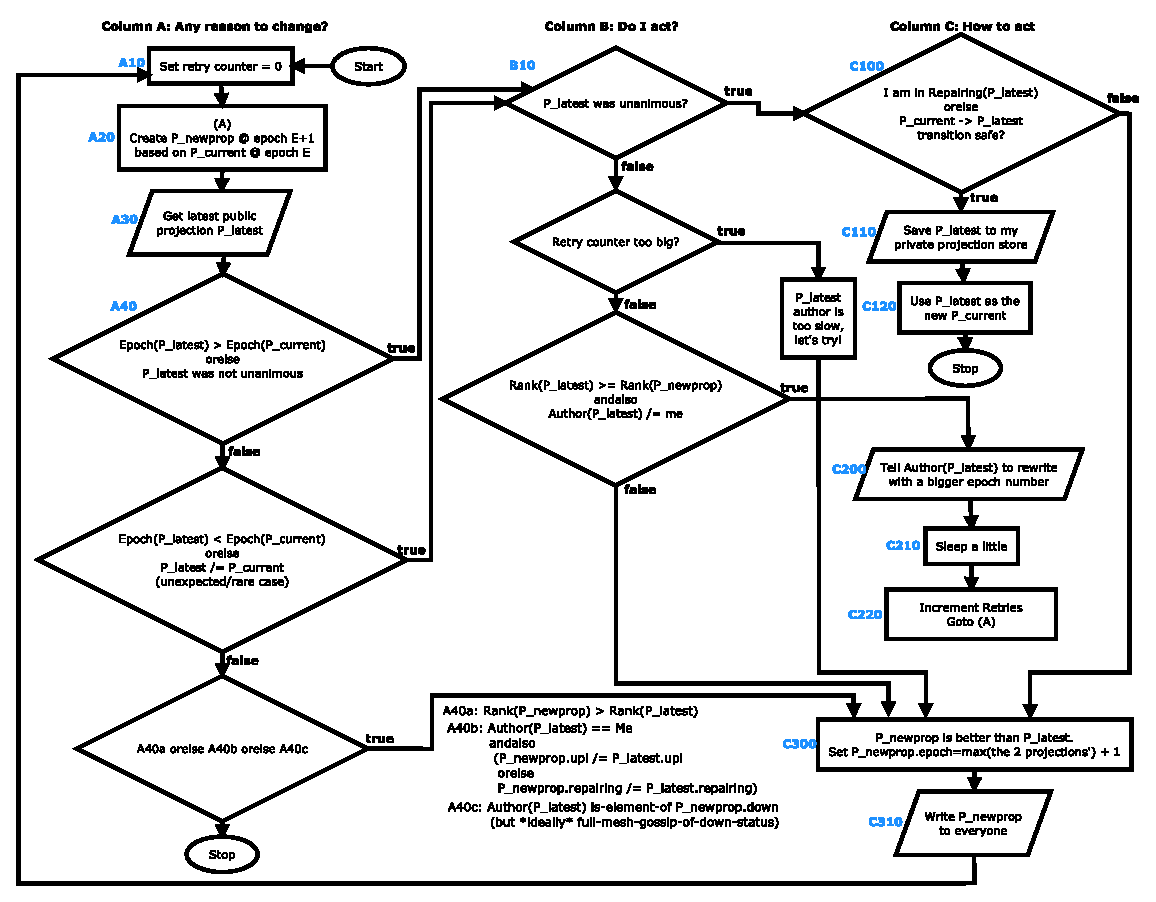
\includegraphics[width=\textwidth]{chain-self-management-sketch.Diagram1.eps}
	}
\caption{Humming consensus flow chart}
\label{fig:flowchart}
\end{figure*}

This section will refer heavily to Figure~\ref{fig:flowchart}, a
flowchart of the humming consensus algorithm.  The following notation
is used by the flowchart and throughout this section.

\begin{description}
\item[Author] The name of the server that created the projection.

\item[Rank] Assigns a numeric score to a projection, see
  Section~\ref{sub:ranking-projections}.

\item[E] The epoch number of a projection.

\item[UPI] "Update Propagation Invariant".  The UPI part of the projection
  is the ordered list of chain members where the UPI is preserved,
  i.e., all UPI list members have their data fully synchronized
  (except for updates in-process at the current instant in time).
  The UPI list is what Chain Replication usually considers ``the
  chain'', i.e., for strongly consistent read operations, all clients
  send their read operations to the tail/last member of the UPI server
  list.
  In Hibari's implementation of Chain Replication
  \cite{cr-theory-and-practice}, the chain members between the
  ``head'' and ``official tail'' (inclusive) are what Machi calls the
  UPI server list.  See also Section~\ref{sub:upi}.

\item[Repairing] The ordered list of nodes that are in repair mode,
  i.e., synchronizing their data with the UPI members of the chain.
  In Hibari's implementation of Chain Replication, any chain members
  that follow the ``official tail'' are what Machi calls the repairing
  server list.

\item[Down] The list of chain members believed to be down, from the
  perspective of the author.

\item[$\mathbf{P_{current}}$] The current projection in active use by the local
  node.  It is also the projection with largest
  epoch number in the local node's private projection store.

\item[$\mathbf{P_{newprop}}$] A new projection suggestion, as
  calculated by the local server
  (Section~\ref{sub:humming-projection-calculation}).

\item[$\mathbf{P_{latest}}$] The highest-ranked projection with the largest
  single epoch number that has been read from all available public
  projection stores, including the local node's public store.

\item[Unanimous] The $P_{latest}$ projections are unanimous if they are
  effectively identical.  Minor differences such as creation time may
  be ignored, but elements such as the UPI list must not be ignored.

\item[$\mathbf{P_{current} \rightarrow P_{latest}}$ transition safe?]
  A predicate function to
  check the sanity \& safety of the transition from the local server's
  $P_{current}$ to the $P_{latest}$ projection.

\item[Stop state] One iteration of the self-management algorithm has
  finished on the local server.
\end{description}

The Erlang source code that implements the Machi chain manager is
structured as a state machine where the function executing for the
flowchart's state is named by the approximate location of the state
within the flowchart.  The flowchart has three columns, from left to
right: 

\begin{description}
\item[Column A] Any reason to change?
\item[Column B] Do I act?
\item[Column C] How do I act?
  \begin{description}
  \item[C1xx] Save latest suggested projection to local private store, unwedge,
    then stop.
  \item[C2xx] Ping author of latest to try again, then wait, then iterate.
  \item[C3xx] The new projection appears best: write
    $P_{newprop}=P_{new}$ to all public projection stores, then iterate.
  \end{description}
\end{description}

Most flowchart states in a column are numbered in increasing order,
top-to-bottom.  These numbers appear in blue in
Figure~\ref{fig:flowchart}.  Some state numbers, such as $A40$,
describe multiple flowchart states; the Erlang code for that function,
e.g. {\tt react\_to\_\-env\_A40()}, implements the logic for all such
flowchart states.

\subsection{Network monitoring}
\label{sub:humming-network-monitoring}

The actions described in this section are executed in the top part of
Column~A of Figure~\ref{fig:flowchart}.
See also, Section~\ref{sub:network-monitoring}.

In today's implementation, there is only a single criterion for
determining the alive/perhaps-not-alive status of a remote server $S$:
is $S$'s projection store available now?  This question is answered by
attemping to use the projection store API on server $S$.  
If successful, then we assume that all
$S$ is available.  If $S$'s projection store is not available for any
reason (including timeout), we assume $S$ is entirely unavailable.
This simple single
criterion appears to be sufficient for humming consensus, according to
simulations of arbitrary network partitions.

%% {\bf NOTE:} The projection store API is accessed via TCP.  The network
%% partition simulator, mentioned above and described at
%% \cite{machi-chain-management-sketch-org}, simulates message drops at
%% the ISO layer 6/7, not IP packets at ISO layer 3.

\subsection{Calculating a new projection data structure}
\label{sub:humming-projection-calculation}

The actions described in this section are executed in the top part of
Column~A of Figure~\ref{fig:flowchart}.
See also, Section~\ref{sub:projection-calculation}.

Execution starts at ``Start'' state of Column~A of
Figure~\ref{fig:flowchart}.  Rule $A20$'s uses recent success \&
failures in accessing other public projection stores to select a hard
boolean up/down status for each participating server.

\subsubsection{Calculating flapping state}

Also at this stage, the chain manager calculates its local
``flapping'' state.  The name ``flapping'' is borrowed from IP network
engineer jargon ``route flapping'':

\begin{quotation}
``Route flapping is caused by pathological conditions
(hardware errors, software errors, configuration errors, intermittent
errors in communications links, unreliable connections, etc.) within
the network which cause certain reachability information to be
repeatedly advertised and withdrawn.''  \cite{wikipedia-route-flapping}
\end{quotation}

\paragraph{Flapping due to constantly changing network partitions and/or server crashes and restarts}

Currently, Machi does not attempt to dampen, smooth, or ignore recent
history of constantly flapping peer servers.  If necessary, a failure
detector such as the $\phi$ accrual failure detector
\cite{phi-accrual-failure-detector} can be used to help mange such
situations.

\paragraph{Flapping due to asymmetric network partitions} TODO needs
some polish

The simulator's behavior during stable periods where at least one node
is the victim of an asymmetric network partition is \ldots weird,
wonderful, and something I don't completely understand yet.  This is
another place where we need more eyes reviewing and trying to poke
holes in the algorithm.

In cases where any node is a victim of an asymmetric network
partition, the algorithm oscillates in a very predictable way: each
server $S$ makes the same $P_{new}$ projection at epoch $E$ that $S$ made
during a previous recent epoch $E-\delta$ (where $\delta$ is small, usually
much less than 10).  However, at least one node makes a suggestion that
makes rough consensus impossible.  When any epoch $E$ is not
acceptable (because some node disagrees about something, e.g.,
which nodes are down),
the result is more new rounds of suggestions.

Because any server $S$'s suggestion isn't any different than $S$'s last
suggestion, the system spirals into an infinite loop of
never-agreed-upon suggestions.  This is \ldots really cool, I think.

From the perspective of $S$'s chain manager, the pattern of this
infinite loop is easy to detect: $S$ inspects the pattern of the last
$L$ projections that it has suggested, e.g., the last 10.
Tiny details such as the epoch number and creation timestamp will
differ, but the major details such as UPI list and repairing list are
the same.

If the major details of the last $L$ projections authored and
suggested by $S$ are the same, then $S$ unilaterally decides that it
is ``flapping'' and enters flapping state.  See
Section~\ref{sub:flapping-state} for additional details.

\subsubsection{When to calculate a new projection}

The Chain Manager schedules a periodic timer to act as a reminder to
calculate a new projection.  The timer interval is typically
0.5--2.0 seconds, if the cluster has been stable.  A client may call an
external API call to trigger a new projection, e.g., if that client
knows that an environment change has happened and wishes to trigger a
response prior to the next timer firing.

It's recommended that the timer interval be staggered according to the
participant ranking rules in Section~\ref{sub:ranking-projections};
higher-ranked servers use shorter timer intervals.  Timer staggering
is not required, but the total amount of churn (as measured by
suggested projections that are ignored or immediately replaced by a
new and nearly-identical projection) is lower with staggered timer.

\subsection{Writing a new projection}
\label{sub:humming-proj-storage-writing}

See also: Section~\ref{sub:proj-storage-writing}.

To focus very specifically about writing a projection,
Figure~\ref{fig:flowchart} shows that writing a private projection is
done by state $C110$ and that writing a public projection is done by
states $C300$ and $C310$.

Broadly speaking, there are a number of decisions made in all three
columns of Figure~\ref{fig:flowchart} to decide if and when any type
of projection should be written at all.  Sometimes, the best action is
to do nothing.

\subsubsection{Column A: Any reason to change?}

The main tasks of the flowchart states in Column~A is to calculate a
new projection $P_{new}$ and perhaps also the inner projection
$P_{new2}$ if we're in flapping mode.  Then we try to figure out which
projection has the greatest merit: our current projection
$P_{current}$, the new projection $P_{new}$, or the latest epoch
$P_{latest}$.  If $P_{current}$ is best, then there's nothing more to
do.

\subsubsection{Column B: Do I act?}

The main decisions that states in Column B need to make are:

\begin{itemize}

\item Is the $P_{latest}$ projection written unanimously (as far as we
  call tell right now)?  If yes, then we out to seriously consider
  using it for our new internal state; go to state $C100$.

\item Is some other server's $P_{latest}$ projection better than my
  $P_{new}$?  If so,
  then we wait for a while.  The waiting loop is broken by a local
  retry counter.  If the counter is small enough, we wait (via state
  $C200$).  While we wait, the author of the better projection will
  hopefully have an opportunity to re-write it in a newer epoch
  unanimously.  If the counter is too big, then we break out and go to
  $C300$.

\item Otherwise we go to state $C300$, where we try to write our
  $P_{new}$ to all public projection stores because, as far as we can
  discern, our projection is best and everyone else ought to know it.

\end{itemize}

It's notable that if $P_{new}$ is truly the best projection available
at the moment, it must always be written unanimously to everyone's
public projection stores and then processed through another
monitor-calculate loop through the flowchart before it can be adopted
via state $C120$.

\subsubsection{Column C: How do I act?}

This column contains three variations of how to act:

\begin{description}

\item[C1xx] Try to adopt the $P_{latest}$ suggestion.  If the transition
  between $P_{current}$ to $P_{latest}$ is completely safe, we'll use
  it by storing it in our local private projection store and then
  adopt it as $P_{current}$.  If it isn't safe, then jump to $C300$.

\item[C2xx] Do nothing but sleep a while.  Then we loop back to state
  $A20$ and step through the flowchart loop again.  Optionally, we
  might want to poke the author of $P_{latest}$ to try again to write
  its proposal unanimously.

\item[C3xx] We try to replicate our $P_{new}$ suggestion to all local
  projection stores, because it seems best.

\end{description}

\subsection{Adopting a new projection}
\label{sub:humming-proj-adoption}

See also: Section~\ref{sub:proj-adoption}.

A new projection $P_E$ is adopted by a Machi server at epoch $E$ if
the following two requirements are met:

\paragraph{\#1: All available copies of $P_E$ are unanimous/identical}

If we query all available servers for their latest projection, then assume
that $E$ is the largest epoch number found.  If we read public
projections for epoch $E$ from all available servers, and if all are
equal to some projection $P_E$, then projection $P_E$ is
(by definition) the best candidate for adoption by the local server.

If we see a projection $P^2_E$ that has the same epoch $E$ but a
different checksum value, then we must consider $P^2_E \ne P_E$.
If we see multiple different values $P^*_E$ for epoch $E$, then the
projection calculation subsystem is notified.  This notification
will trigger a calculation of a new projection $P_{E+1}$ which
may eventually be stored and therefore help
resolve epoch $E$'s ambiguous and unusable condition.

\paragraph{\#2: The transition from current $\rightarrow$ new projection is
safe}

The projection $P_E = P_{latest}$ is evaluated by numerous rules and
invariants, relative to the projection that the server is currently
using, $P_{current}$.  If such rule or invariant is violated/false,
then the local server will discard $P_{latest}$.  Instead, it will
trigger the projection calculation subsystem to create an alternative,
safe projection $P_{latest+1}$ that will hopefully create a unanimous
epoch $E+1$.

The transition from $P_{current} \rightarrow P_{latest}$ is checked
for safety and sanity.  The conditions used for the check include:

\begin{enumerate}
\item The Erlang data types of all record members are correct.
\item UPI, down, and repairing lists contain no duplicates and are in fact
   mutually disjoint.
\item The author node is not down (as far as we can tell).
\item Any server $N$ that was added to $P_{latest}$'s UPI list must
  appear in the tail the UPI list, and $N$ must have been in
  $P_{current}$'s repairing list.
\item No re-ordering of the UPI list members: any server $S$ that is
  in $P_{latest}$'s UPI list that was not present in $P_{current}$'s
  UPI list must in the same position as it appeared in $P_{current}$'s
  UPI list.  The same re-reordering restriction applies to all
  servers in $P_{latest}$'s repairing list relative to
  $P_{current}$'s repairing list.
\end{enumerate}

The safety check may be performed pair-wise once or pair-wise across
the entire history sequence of a server/FLU's private projection
store.

\subsection{Additional discussion of flapping state}
\label{sub:flapping-state}
All $P_{new}$ projections
calculated while in flapping state have additional diagnostic
information added, including:

\begin{itemize}
\item Flag: server $S$ is in flapping state
\item Epoch number \& wall clock timestamp when $S$ entered flapping state
\item The collection of all other known participants who are also
  flapping (with respective starting epoch numbers).
\item A list of nodes that are suspected of being partitioned, called the
  ``hosed list''.  The hosed list is a union of all other hosed list
  members that are ever witnessed, directly or indirectly, by a server
  while in flapping state.
\end{itemize}

\subsubsection{Flapping diagnostic data accumulates}

While in flapping state, this diagnostic data is gathered from
all available participants and merged together in a CRDT-like manner.
Once added to the diagnostic data list, a datum remains until
$S$ drops out of flapping state.  When flapping state stops, all
accumulated diagnostic data is discarded.

This accumulation of diagnostic data in the projection data
structure acts in part as a substitute for a gossip protocol.
However, since all participants are already communicating with each
other via read \& writes to each others' projection stores, this
data can propagate in a gossip-like manner via projections.  If
this is insufficient, then a more gossip'y protocol can be used to
distribute flapping diagnostic data.

\subsubsection{Flapping example}
\label{ssec:flapping-example}

Any server listed in the ``hosed list'' is suspected of having some
kind of network communication problem with some other server.  For
example, let's examine a scenario involving a Machi cluster of servers
$a$, $b$, $c$, $d$, and $e$.  Assume there exists an asymmetric network
partition such that messages from $a \rightarrow b$ are dropped, but
messages from $b \rightarrow a$ are delivered.\footnote{If this
  partition were happening at or before the level of a reliable
  delivery protocol like TCP, then communication in {\em both}
  directions would be affected.  However, in this model, we are
  assuming that the ``messages'' lost in partitions are projection API
  call operations and their responses.}

Once a participant $S$ enters flapping state, it starts gathering the
flapping starting epochs and hosed lists from all of the other
projection stores that are available.  The sum of this info is added
to all projections calculated by $S$.
For example, projections authored by $a$ will say that $a$ believes
that $b$ is down. 
Likewise, projections authored by $b$ will say that $b$ believes
that $a$ is down. 

\subsubsection{The inner projection}
\label{ssec:inner-projection}

We continue the example started in the previous subsection\ldots.

Eventually, in a gossip-like manner, all other participants will
eventually find that their hosed list is equal to $[a,b]$.  Any other
server, for example server $c$, will then calculate another
projection, $P_{new2}$, using the assumption that both $a$ and $b$
are down.

\begin{itemize}
\item If operating in the default CP mode, both $a$ and $b$ are down
  and therefore not eligible to participate in Chain Replication.
  %% The chain may continue service if a $c$, $d$, $e$ and/or witness
  %% servers can try to form a correct UPI list for the chain.
  This may cause an availability problem for the chain: we may not
  have a quorum of participants (real or witness-only) to form a
  correct UPI chain.
\item If operating in AP mode, $a$ and $b$ can still form two separate
  chains of length one, using UPI lists of $[a]$ and $[b]$, respectively. 
\end{itemize}

This re-calculation, $P_{new2}$, of the new projection is called an
``inner projection''.  This inner projection definition is nested
inside of its parent projection, using the same flapping disagnostic
data used for other flapping status tracking.

When humming consensus has determined that a projection state change
is necessary and is also safe, then the outer projection is written to
the local private projection store.
With respect to future iterations of
humming consensus, regardless of flapping state, the outer projection
is always used.
However, the server's subsequent
behavior with respect to Chain Replication will be relative to the
{\em inner projection only}.  The inner projection is used to trigger
wedge/un-wedge behavior as well as being the projection that is
advertised to Machi clients.

The epoch of the inner projection, $E^{inner}$ is always less than or
equal to the epoch of the outer projection, $E$.  The $E^{inner}$
epoch typically only changes when new servers are added to the hosed
list.

To attempt a rough analogy, the outer projection is the carrier wave
that is used to transmit the information of the inner projection.

\subsubsection{Outer projection churn, inner projection stability}

One of the intriguing features of humming consensus's reaction to
asymmetric partition: flapping behavior continues for as long as
an any asymmetric partition exists.

\subsubsection{Leaving flapping state and discarding inner projectino}

There are two events that can trigger leaving flapping state.

\begin{itemize}

\item A server $S$ in flapping state notices that its long history of
  repeatedly suggesting the same $P_{new}=X$ projection will be broken:
  $S$ instead calculates some differing projection $P_{new} = Y$ instead.
  This change in projection history happens whenever the network
  partition changes in a significant way.

\item Server $S$ reads a public projection, $P_{noflap}$, that is
  authored by another server $S'$, and that $P_{noflap}$ no longer
  contains the flapping start epoch for $S'$ that is present in the
  history that $S$ has maintained of all projection history while in
  flapping state.

\end{itemize}

When either event happens, server $S$ will exit flapping state.  All
new projections authored by $S$ will have all flapping diagnostic data
removed.  This includes stopping use of the inner projection: the UPI
list of the inner projection is copied to the outer projection's UPI
list, to avoid a drastic change in UPI membership.

\subsubsection{Stability in symmetric partition cases}

Although humming consensus hasn't been formally proven to handle all
asymmetric and symmetric partition cases, the current implementation
appears to converge rapidly to a single chain state in all symmetric
partition cases.  This is in contract to asymmetric partition cases,
where ``flapping'' will continue on every humming consensus iteration
until all asymmetric partition disappears.  Such proof is an area of
future work.

\subsection{Ranking projections}
\label{sub:ranking-projections}

A projection's rank is based on the epoch number (higher always wins),
chain length (larger wins), number \& state of any repairing members
of the chain (larger wins), and node name of the author server (as a
tie-breaking criteria).

\section{``Split brain'' management in CP Mode}
\label{sec:split-brain-management}

Split brain management is a thorny problem.  The method presented here
is one based on pragmatics.  If it doesn't work, there isn't a serious
worry, because Machi's first serious use case all require only AP Mode.
If we end up falling back to ``use Riak Ensemble'' or ``use ZooKeeper'',
then perhaps that's
fine enough.  Meanwhile, let's explore how a
completely self-contained, no-external-dependencies
CP Mode Machi might work.

Wikipedia's description of the quorum consensus solution\footnote{See
  {\tt http://en.wikipedia.org/wiki/Split-brain\_(computing)}.} is nice
and short:

\begin{quotation}
A typical approach, as described by Coulouris et al.,[4] is to use a
quorum-consensus approach. This allows the sub-partition with a
majority of the votes to remain available, while the remaining
sub-partitions should fall down to an auto-fencing mode.
\end{quotation}

This is the same basic technique that
both Riak Ensemble and ZooKeeper use.  Machi's
extensive use of write-registers are a big advantage when implementing
this technique.  Also very useful is the Machi ``wedge'' mechanism,
which can automatically implement the ``auto-fencing'' that the
technique requires.  All Machi servers that can communicate with only
a minority of other servers will automatically ``wedge'' themselves
and refuse all requests for service until communication with the
majority can be re-established.

\subsection{The quorum: witness servers vs. full servers}

In any quorum-consensus system, at least $2f+1$ participants are
required to survive $f$ participant failures.  Machi can implement a
technique of ``witness servers'' servers to bring the total cost
somewhere in the middle, between $2f+1$ and $f+1$, depending on your
point of view.

A ``witness server'' is one that participates in the network protocol
but does not store or manage all of the state that a ``full server''
does.  A ``full server'' is a Machi server as
described by this RFC document.  A ``witness server'' is a server that
only participates in the projection store and projection epoch
transition protocol and a small subset of the file access API.
A witness server doesn't actually store any
Machi files.  A witness server is almost stateless, when compared to a
full Machi server.

A mixed cluster of witness and full servers must still contain at
least $2f+1$ participants.  However, only $f+1$ of them are full
participants, and the remaining $f$ participants are witnesses.  In
such a cluster, any majority quorum must have at least one full server
participant.

Witness servers are always placed at the front of the chain.  As stated
above, there may be at most $f$ witness servers.  A functioning quorum
majority
must have at least $f+1$ servers that can communicate and therefore
calculate and store a new unanimous projection.  Therefore, any server at
the tail of a functioning quorum majority chain must be full server.  Full servers
actually store Machi files, so they have no problem answering {\tt
  read\_req} API requests.\footnote{We hope that it is now clear that
  a witness server cannot answer any Machi file read API request.}

Any server that can only communicate with a minority of other servers will
find that none can calculate a new projection that includes a
majority of servers.  Any such server, when in CP mode, would then move to
wedge state and remain wedged until the network partition heals enough
to communicate with the majority side.  This is a nice property: we
automatically get ``fencing'' behavior.\footnote{Any server on the minority side
  is wedged and therefore refuses to serve because it is, so to speak,
  ``on the wrong side of the fence.''}

There is one case where ``fencing'' may not happen: if both the client
and the tail server are on the same minority side of a network partition.
Assume the client and server $S_z$ are on the "wrong side" of a network
split; both are using projection epoch $P_1$.  The tail of the
chain is $S_z$.

Also assume that the "right side" has reconfigured and is using
projection epoch $P_2$.  The right side has mutated key $K$.  Meanwhile,
nobody on the "right side" has noticed anything wrong and is happy to
continue using projection $P_1$.

\begin{itemize}
\item {\bf Option a}: Now the wrong side client reads $K$ using $P_1$ via
  $S_z$.  $S_z$ does not detect an epoch problem and thus returns an
  answer.  Given our assumptions, this value is stale.  For some
  client use cases, this kind of staleness may be OK in trade for
  fewer network messages per read \ldots so Machi may
  have a configurable option to permit it.
\item {\bf Option b}: The wrong side client must confirm that $P_1$ is
  in use by a full majority of chain members, including $S_z$.
\end{itemize}

Attempts using Option b will fail for one of two reasons.  First, if
the client can talk to a server that is using $P_2$, the client's
operation must be retried using $P_2$.  Second, the client will time
out talking to enough servers so that it fails to get a quorum's worth of
$P_1$ answers.  In either case, Option B will always fail a client
read and thus cannot return a stale value of $K$.

\subsection{Witness server data and protocol changes}

Some small changes to the projection's data structure
are required (relative to the initial spec described in
\cite{machi-design}).  The projection itself
needs new annotation to indicate the operating mode, AP mode or CP
mode.  The state type notifies the chain manager how to
react in network partitions and how to calculate new, safe projection
transitions and which file repair mode to use
(Section~\ref{sec:repair-entire-files}).
Also, we need to label member server servers as full- or
witness-type servers.

Write API requests are processed by witness servers in {\em almost but
  not quite} no-op fashion.  The only requirement of a witness server
is to return correct interpretations of local projection epoch
numbers, via the {\tt error\_bad\_epoch} and {\tt error\_wedged} error
codes.  In fact, a new API call is sufficient for querying witness
servers: {\tt \{check\_epoch, m\_epoch()\}}.
Any client write operation sends the {\tt
  check\_\-epoch} API command to witness servers and sends the usual {\tt
  write\_\-req} command to full servers.

\subsection{Restarting after entire chain crashes}

TODO This is $1^{st}$ draft of this section.

There's a corner case that requires additional safety checks to
preserve strong consistency: restarting after the entire chain crashes.

The default restart behavior for the chain manager is to start the
local server $S$ with $P_{current} = P_{zero}$, i.e., $S$
believes that the current chain length is zero.  Then $S$'s chain
manager will attempt to join the chain by waiting for another active
chain member $S'$ to notice that $S$ is now available.  Then $S'$'s
chain manager will automatically suggest a projection where $S$ is
added to the repairing list.  If there is no other active server $S'$,
then $S$ will suggest projection $P_{one}$, a chain of length one
where $S$ is the sole UPI member of the chain.

The default restart strategy cannot work correctly if: a). all members
of the chain crash simultaneously (e.g., power failure), and b). the UPI
chain was not at maximum length (i.e., no chain members are under
repair or down).  For example, assume that the cluster consists of
servers $S_a$ and $S_b$, and the UPI chain is $P_{one} = [S_a]$ when a power
failure terminates the entire data center.  Assume that when power is
restored, server $S_b$ restarts first.  $S_b$'s chain manager must not
suggest $P_{one} = [S_b]$ --- we do not know how much stale data $S_b$
might have, but clients must not access $S_b$ at thsi time.

The correct course of action in this crash scenario is to wait until
$S_a$ returns to service.  In general, however, we have to wait until
a quorum of servers (including witness servers) have restarted to
determine the last operational state of the cluster.  This operational
history is preserved and distributed amongst the participants' private
projection stores.

\section{Possible problems with Humming Consensus}

There are some unanswered questions about Machi's proposed chain
management technique.  The problems that we guess are likely/possible
include:

\begin{itemize}

\item Coping with rare flapping conditions.
  It's hoped that the ``best projection'' ranking system
  will be sufficient to prevent endless flapping of projections, but
  it isn't yet clear that it will be.

\item CP Mode management via the method proposed in
  Section~\ref{sec:split-brain-management} may not be sufficient in
  all cases.

\end{itemize}

\section{Repair of entire files}
\label{sec:repair-entire-files}

There are some situations where repair of entire files is necessary.

\begin{itemize}
\item To repair servers added to a chain in a projection change,
  specifically adding a new server to the chain.  This case covers both
  adding a new, data-less server and re-adding a previous, data-full server
  back to the chain.
\item To avoid data loss when changing the order of the chain's servers.
\end{itemize}

Both situations can set the stage for data loss in the future.
If a violation of the Update Propagation Invariant (see end of
Section~\ref{sec:cr-proof}) is permitted, then the strong consistency
guarantee of Chain Replication is violated.  Because Machi uses
write-once registers, the number of possible strong consistency
violations is small: any client that witnesses a written $\rightarrow$
unwritten transition is a violation of strong consistency.  But
avoiding even this one bad scenario is a bit tricky.

Data
unavailability/loss when all chain servers fail is unavoidable.  We
wish to avoid data loss whenever a chain has at least one surviving
server.  Another method to avoid data loss is to preserve the Update
Propagation Invariant at all times.

\subsection{Just ``rsync'' it!}
\label{ssec:just-rsync-it}

A simple repair method might be perhaps 90\% sufficient.
That method could loosely be described as ``just {\tt rsync}
all files to all servers in an infinite loop.''\footnote{The
  file format suggested in
  \cite{machi-design} does not permit {\tt rsync}
  as-is to be sufficient.  A variation of {\tt rsync} would need to be
  aware of the data/metadata split within each file and only replicate
  the data section \ldots and the metadata would still need to be
  managed outside of {\tt rsync}.}

However, such an informal method
cannot tell you exactly when you are in danger of data loss and when
data loss has actually happened.  If we maintain the Update
Propagation Invariant, then we know exactly when data loss is immanent
or has happened.

Furthermore, we hope to use Machi for multiple use cases, including
ones that require strong consistency.
For uses such as CORFU, strong consistency is a non-negotiable
requirement.  Therefore, we will use the Update Propagation Invariant
as the foundation for Machi's data loss prevention techniques.

\subsection{Divergence from CORFU: repair}
\label{sub:repair-divergence}

The original repair design for CORFU is simple and effective,
mostly.  See Figure~\ref{fig:corfu-style-repair} for a full
description of the algorithm
Figure~\ref{fig:corfu-repair-sc-violation} for an example of a strong
consistency violation that can follow.  (NOTE: This is a variation of
the data loss scenario that is described in
Figure~\ref{fig:data-loss2}.)

\begin{figure}
\begin{enumerate}
\item Destroy all data on the repair destination FLU.
\item Add the repair destination FLU to the tail of the chain in a new
  projection $P_{p+1}$.
\item Change projection from $P_p$ to $P_{p+1}$.
\item Let single item read repair fix all of the problems.
\end{enumerate}
\caption{Simplest CORFU-style repair algorithm.}
\label{fig:corfu-style-repair}
\end{figure}

\begin{figure}
\begin{enumerate}
\item Write value $V$ to offset $O$ in the log with chain $[S_a]$.
  This write is considered successful.
\item Change projection to configure chain as $[S_a,S_b]$.  Prior to
  the change, all values on FLU $S_b$ are unwritten.
\item FLU server $S_a$ crashes.  The new projection defines the chain
  as $[S_b]$.
\item A client attempts to read offset $O$ and finds an unwritten
  value.  This is a strong consistency violation.
%% \item The same client decides to fill $O$ with the junk value
%%   $V_{junk}$.  Now value $V$ is lost.
\end{enumerate}
\caption{An example scenario where the CORFU simplest repair algorithm
  can lead to a violation of strong consistency.}
\label{fig:corfu-repair-sc-violation}
\end{figure}

\begin{figure}
\begin{enumerate}
\item Projection $P_p$ says that chain membership is $[S_a]$.
\item A write of data $D$ to file $F$ at offset $O$ is successful.
\item Projection $P_{p+1}$ says that chain membership is $[S_a,S_b]$, via
   an administration API request.
\item Machi will trigger repair operations, copying any missing data
   files from FLU $S_a$ to FLU $S_b$.  For the purpose of this
   example, the sync operation for file $F$'s data and metadata has
   not yet started.
\item FLU $S_a$ crashes.
\item The chain manager on $S_b$ notices $S_a$'s crash,
   decides to create a new projection $P_{p+2}$ where chain membership is
   $[S_b]$
  successfully stores $P_{p+2}$ in its local store.  FLU $S_b$ is now wedged.
\item FLU $S_a$ is down, therefore the
   value of $P_{p+2}$ is unanimous for all currently available FLUs
   (namely $[S_b]$).
\item FLU $S_b$ sees that projection $P_{p+2}$ is the newest unanimous
   projection.  It unwedges itself and continues operation using $P_{p+2}$.
\item Data $D$ is definitely unavailable for now.  If server $S_a$ is
  never re-added to the chain, then data $D$ is lost forever.
\end{enumerate}
\caption{Data unavailability scenario with danger of permanent data loss}
\label{fig:data-loss2}
\end{figure}

A variation of the repair
algorithm is presented in section~2.5 of a later CORFU paper \cite{corfu2}.
However, the re-use a failed
server is not discussed there, either: the example of a failed server
$S_6$ uses a new server, $S_8$ to replace $S_6$.  Furthermore, the
repair process is described as:

\begin{quote}
``Once $S_6$ is completely rebuilt on $S_8$ (by copying entries from
  $S_7$), the system moves to projection (C), where $S_8$ is now used
  to service all reads in the range $[40K,80K)$.''
\end{quote}

The phrase ``by copying entries'' does not give enough
detail to avoid the same data race as described in
Figure~\ref{fig:corfu-repair-sc-violation}.  We believe that if
``copying entries'' means copying only written pages, then CORFU
remains vulnerable.  If ``copying entries'' also means ``fill any
unwritten pages prior to copying them'', then perhaps the
vulnerability is eliminated.\footnote{SLF's note: Probably?  This is my
  gut feeling right now.  However, given that I've just convinced
  myself 100\% that fill during any possibility of split brain is {\em
  not safe} in Machi, I'm not 100\% certain anymore than this ``easy''
  fix for CORFU is correct.}.

\subsection{Whole file repair as servers are (re-)added to a chain}
\label{sub:repair-add-to-chain}

\begin{figure*}
\centering
$
[\overbrace{\underbrace{H_1}_\textbf{Head of Heads}, M_{11},
      \underbrace{T_1}_\textbf{Tail \#1}}^\textbf{Chain \#1 (U.P.~Invariant preserving)}
\mid
\overbrace{H_2, M_{21},
      \underbrace{T_2}_\textbf{Tail \#2}}^\textbf{Chain \#2 (repairing)}
\mid \ldots \mid
\overbrace{H_n, M_{n1},
      \underbrace{T_n}_\textbf{Tail \#n \& Tail of Tails ($T_{tails}$)}}^\textbf{Chain \#n (repairing)}
]
$
\caption{Representation of a ``chain of chains'': a chain prefix of
  Update Propagation Invariant preserving FLUs (``Chain \#1'')
  with FLUs from $n-1$ other chains under repair.}
\label{fig:repair-chain-of-chains}
\end{figure*}

\begin{figure}
\centering
$
[\overbrace{\underbrace{H_1}_\textbf{Head}, M_{11}, T_1,
                        H_2, M_{21}, T_2,
                        \ldots
                        H_n, M_{n1},
                        \underbrace{T_n}_\textbf{Tail}}^\textbf{Chain (U.P.~Invariant preserving)}
]
$
\caption{Representation of Figure~\ref{fig:repair-chain-of-chains}
  after all repairs have finished successfully and a new projection has
  been calculated.}
\label{fig:repair-chain-of-chains-finished}
\end{figure}

Machi's repair process must preserve the Update Propagation
Invariant.  To avoid data races with data copying from
``U.P.~Invariant preserving'' servers (i.e. fully repaired with
respect to the Update Propagation Invariant)
to servers of unreliable/unknown state, a
projection like the one shown in
Figure~\ref{fig:repair-chain-of-chains} is used.  In addition, the
operations rules for data writes and reads must be observed in a
projection of this type.

\begin{itemize}

\item The system maintains the distinction between ``U.P.~preserving''
  and ``repairing'' FLUs at all times.  This allows the system to
  track exactly which servers are known to preserve the Update
  Propagation Invariant and which servers may/may not.

\item All ``repairing'' FLUs must be added only at the end of the
  chain-of-chains.

\item All write operations must flow successfully through the
  chain-of-chains from beginning to end, i.e., from the ``head of
  heads'' to the ``tail of tails''.  This rule also includes any
  repair operations.

\item In AP Mode, all read operations are attempted from the list of
$[T_1,\-T_2,\-\ldots,\-T_n]$, where these FLUs are the tails of each of the
chains involved in repair.
In CP mode, all read operations are attempted only from $T_1$.
The first reply of {\tt \{ok, <<...>>\}} is a correct answer;
the rest of the FLU list can be ignored and the result returned to the
client.  If all FLUs in the list have an unwritten value, then the
client can return {\tt error\_unwritten}.

\end{itemize}

While the normal single-write and single-read operations are performed
by the cluster, a file synchronization process is initiated.  The
sequence of steps differs depending on the AP or CP mode of the system.

\subsubsection{Repair in CP mode}

In cases where the cluster is operating in CP Mode,
CORFU's repair method of ``just copy it all'' (from source FLU to repairing
FLU) is correct, {\em except} for the small problem pointed out in
Section~\ref{sub:repair-divergence}.  The problem for Machi is one of
time \& space.  Machi wishes to avoid transferring data that is
already correct on the repairing nodes.  If a Machi node is storing
20TBytes of data, we really do not wish to use 20TBytes of bandwidth
to repair only 1 GByte of truly-out-of-sync data.

However, it is {\em vitally important} that all repairing FLU data be
clobbered/overwritten with exactly the same data as the Update
Propagation Invariant preserving chain.  If this rule is not strictly
enforced, then fill operations can corrupt Machi file data.  The
algorithm proposed is:

\begin{enumerate}

\item Change the projection to a ``chain of chains'' configuration
  such as depicted in Figure~\ref{fig:repair-chain-of-chains}.

\item For all files on all FLUs in all chains, extract the lists of
  written/unwritten byte ranges and their corresponding file data
  checksums.  (The checksum metadata is not strictly required for
  recovery in AP Mode.)
  Send these lists to the tail of tails
  $T_{tails}$, which will collate all of the lists into a list of
  tuples such as {\tt \{FName, $O_{start}, O_{end}$, CSum, FLU\_List\}}
  where {\tt FLU\_List} is the list of all FLUs in the entire chain of
  chains where the bytes at the location {\tt \{FName, $O_{start},
    O_{end}$\}} are known to be written (as of the current repair period).

\item For chain \#1 members, i.e., the
  leftmost chain relative to Figure~\ref{fig:repair-chain-of-chains},
  repair files byte ranges for any chain \#1 members that are not members
  of the {\tt FLU\_List} set.  This will repair any partial
  writes to chain \#1 that were unsuccessful (e.g., client crashed).
  (Note however that this step only repairs FLUs in chain \#1.)

\item For all file byte ranges in all files on all FLUs in all
  repairing chains where Tail \#1's value is unwritten, force all
  repairing FLUs to also be unwritten.

\item For file byte ranges in all files on all FLUs in all repairing
  chains where Tail \#1's value is written, send repair file byte data
  \& metadata to any repairing FLU if the value repairing FLU's
  value is unwritten or the checksum is not exactly equal to Tail \#1's
  checksum.

\end{enumerate}

When the repair is known to have copied all missing data successfully,
then the chain can change state via a new projection that includes the
repaired FLU(s) at the end of the U.P.~Invariant preserving chain \#1
in the same order in which they appeared in the chain-of-chains during
repair.  See Figure~\ref{fig:repair-chain-of-chains-finished}.

The repair can be coordinated and/or performed by the $T_{tails}$ FLU
or any other FLU or cluster member that has spare capacity.

There is no serious race condition here between the enumeration steps
and the repair steps.  Why?  Because the change in projection at
step \#1 will force any new data writes to adapt to a new projection.
Consider the mutations that either happen before or after a projection
change:

\begin{itemize}

\item For all mutations $M_1$ prior to the projection change, the
  enumeration steps \#3 \& \#4 and \#5 will always encounter mutation
  $M_1$.  Any repair must write through the entire chain-of-chains and
  thus will preserve the Update Propagation Invariant when repair is
  finished.

\item For all mutations $M_2$ starting during or after the projection
  change has finished, a new mutation $M_2$ may or may not be included in the
  enumeration steps \#3 \& \#4 and \#5.
  However, in the new projection, $M_2$ must be
  written to all chain of chains members, and such
  in-order writes will also preserve the Update
  Propagation Invariant and therefore is also be safe.

\end{itemize}

\subsubsection{Repair in AP Mode}

In cases the cluster is operating in AP Mode:

\begin{enumerate}
\item Follow the first two steps of the ``CP Mode''
  sequence (above).
\item Follow step \#3 of the ``strongly consistent mode'' sequence
  (above), but in place of repairing only FLUs in Chain \#1, AP mode
  will repair the byte range of any FLU that is not a member of the
  {\tt FLU\_List} set.
\item End of procedure.
\end{enumerate}

The end result is a huge ``merge'' where any
{\tt \{FName, $O_{start}, O_{end}$\}} range of bytes that is written
on FLU $S_w$ but missing/unwritten from FLU $S_m$ is written down the full chain
of chains, skipping any FLUs where the data is known to be written.
Such writes will also preserve Update Propagation Invariant when
repair is finished.

\subsection{Whole-file repair when changing server ordering within a chain}
\label{sub:repair-chain-re-ordering}

This section has been cut --- please see Git commit history for discussion.

\section{Chain Replication: why is it correct?}
\label{sec:cr-proof}

See Section~3 of \cite{chain-replication} for a proof of the
correctness of Chain Replication.  A short summary is provide here.
Readers interested in good karma should read the entire paper.

\subsection{The Update Propagation Invariant}
\label{sub:upi}

``Update Propagation Invariant'' is the original chain replication
paper's name for the
$H_i \succeq H_j$
property mentioned in Figure~\ref{tab:chain-order}.
This paper will use the same name.
This property may also be referred to by its acronym, ``UPI''.

\subsection{Chain Replication and strong consistency}

The basic rules of Chain Replication and its strong
consistency guarantee:

\begin{enumerate}

\item All replica servers are arranged in an ordered list $C$.

\item All mutations of a datum are performed upon each replica of $C$
  strictly in the order which they appear in $C$.  A mutation is considered
  completely successful if the writes by all replicas are successful.

\item The head of the chain makes the determination of the order of
  all mutations to all members of the chain.  If the head determines
  that some mutation $M_i$ happened before another mutation $M_j$,
  then mutation $M_i$ happens before $M_j$ on all other members of
  the chain.\footnote{While necesary for general Chain Replication,
    Machi does not need this property.  Instead, the property is
    provided by Machi's sequencer and the write-once register of each
    byte in each file.}

\item All read-only operations are performed by the ``tail'' replica,
  i.e., the last replica in $C$.

\end{enumerate}

The basis of the proof lies in a simple logical trick, which is to
consider the history of all operations made to any server in the chain
as a literal list of unique symbols, one for each mutation.

Each replica of a datum will have a mutation history list.  We will
call this history list $H$. For the $i^{th}$ replica in the chain list
$C$, we call $H_i$ the mutation history list for the $i^{th}$ replica.

Before the $i^{th}$ replica in the chain list begins service, its mutation
history $H_i$ is empty, $[]$.  After this replica runs in a Chain
Replication system for a while, its mutation history list grows to
look something like 
$[M_0, M_1, M_2, ..., M_{m-1}]$ where $m$ is the total number of
mutations of the datum that this server has processed successfully.

Let's assume for a moment that all mutation operations have stopped.
If the order of the chain was constant, and if all mutations are
applied to each replica in the chain's order, then all replicas of a
datum will have the exact same mutation history: $H_i = H_J$ for any
two replicas $i$ and $j$ in the chain
(i.e., $\forall i,j \in C, H_i = H_J$).  That's a lovely property,
but it is much more interesting to assume that the service is
not stopped.  Let's look next at a running system.

\begin{figure*}
\centering
\begin{tabular}{ccc}
{\bf {{On left side of $C$}}} & & {\bf On right side of $C$} \\
\hline
\multicolumn{3}{l}{Looking at replica order in chain $C$:} \\
$i$ & $<$ & $j$ \\

\multicolumn{3}{l}{For example:} \\

0 & $<$ & 2 \\
\hline
\multicolumn{3}{l}{It {\em must} be true: history lengths per replica:} \\
length($H_i$) & $\geq$ & length($H_j$) \\
\multicolumn{3}{l}{For example, a quiescent chain:} \\
length($H_i$) = 48 & $\geq$ & length($H_j$) = 48 \\
\multicolumn{3}{l}{For example, a chain being mutated:} \\
length($H_i$) = 55 & $\geq$ & length($H_j$) = 48 \\
\multicolumn{3}{l}{Example ordered mutation sets:} \\
$[M_0,M_1,\ldots,M_{46},M_{47},\ldots,M_{53},M_{54}]$ & $\supset$ & $[M_0,M_1,\ldots,M_{46},M_{47}]$ \\
\multicolumn{3}{c}{\bf Therefore the right side is always an ordered
  subset} \\
\multicolumn{3}{c}{\bf of the left side.  Furthermore, the ordered
  sets on both} \\
\multicolumn{3}{c}{\bf sides have the exact same order of those elements they have in common.} \\
\multicolumn{3}{c}{The notation used by the Chain Replication paper is
shown below:} \\
$[M_0,M_1,\ldots,M_{46},M_{47},\ldots,M_{53},M_{54}]$ & $\succeq$ & $[M_0,M_1,\ldots,M_{46},M_{47}]$ \\

\end{tabular}
\caption{The ``Update Propagation Invariant'' as
  illustrated by Chain Replication protocol history.}
\label{tab:chain-order}
\end{figure*}

If the entire chain $C$ is processing any number of concurrent
mutations, then we can still understand $C$'s behavior.
Figure~\ref{tab:chain-order} shows us two replicas in chain $C$:
replica $R_i$ that's on the left/earlier side of the replica chain $C$
than some other replica $R_j$.  We know that $i$'s position index in
the chain is smaller than $j$'s position index, so therefore $i < j$.
The restrictions of Chain Replication make it true that length($H_i$)
$\ge$ length($H_j$) because it's also that $H_i \supset H_j$, i.e,
$H_i$ on the left is always is a superset of $H_j$ on the right.

When considering $H_i$ and $H_j$ as strictly ordered lists, we have 
$H_i \succeq H_j$, where the right side is always an exact prefix of the left
side's list.  This prefixing propery is exactly what strong
consistency requires.  If a value is read from the tail of the chain,
then no other chain member can have a prior/older value because their
respective mutations histories cannot be shorter than the tail
member's history.

\section{Additional sources for information about humming consensus}

\begin{itemize}
\item ``On Consensus and Humming in the IETF'' \cite{rfc-7282}, for
background on the use of humming by IETF meeting participants during
IETF meetings.

\item ``On `Humming Consensus', an allegory'' \cite{humming-consensus-allegory},
for an allegory in homage to the style of Leslie Lamport's original Paxos
paper.
\end{itemize}

\section{Acknowledgements}

We wish to thank everyone who has read and/or reviewed this document
in its really-terrible early drafts and have helped improve it
immensely: Justin Sheehy, Kota Uenishi, Shunichi Shinohara, Andrew
Stone, Jon Meredith, Chris Meiklejohn, Mark Allen, and Zeeshan
Lakhani.

\bibliographystyle{abbrvnat}
\begin{thebibliography}{}
\softraggedright

\bibitem{elastic-chain-replication}
Abu-Libdeh, Hussam et al.
Leveraging Sharding in the Design of Scalable Replication Protocols.
Proceedings of the 4th Annual Symposium on Cloud Computing (SOCC'13), 2013.
{\tt http://www.ymsir.com/papers/sharding-socc.pdf}

\bibitem{corfu1}
Balakrishnan, Mahesh et al.
CORFU: A Shared Log Design for Flash Clusters.
Proceedings of the 9th USENIX Conference on Networked Systems Design
and Implementation (NSDI'12), 2012.
{\tt http://research.microsoft.com/pubs/157204/ corfumain-final.pdf}

\bibitem{corfu2}
Balakrishnan, Mahesh et al.
CORFU: A Distributed Shared Log
ACM Transactions on Computer Systems, Vol. 31, No. 4, Article 10, December 2013.
{\tt http://www.snookles.com/scottmp/corfu/ corfu.a10-balakrishnan.pdf}

\bibitem{machi-chain-management-sketch-org}
Basho Japan KK.
Machi Chain Self-Management Sketch
{\tt https://github.com/basho/machi/tree/ master/doc/chain-self-management-sketch.org}

\bibitem{machi-design}
Basho Japan KK.
Machi: an immutable file store
{\tt https://github.com/basho/machi/tree/ master/doc/high-level-machi.pdf}

\bibitem{was}
Calder, Brad et al.
Windows Azure Storage: A Highly Available Cloud Storage Service with Strong Consistency
Proceedings of the 23rd ACM Symposium on Operating Systems Principles (SOSP'11), 2011.
{\tt http://sigops.org/sosp/sosp11/current/ 2011-Cascais/printable/11-calder.pdf}

\bibitem{cr-theory-and-practice}
Fritchie, Scott Lystig.
Chain Replication in Theory and in Practice.
Proceedings of the 9th ACM SIGPLAN Workshop on Erlang (Erlang'10), 2010.
{\tt http://www.snookles.com/scott/publications/ erlang2010-slf.pdf}

\bibitem{humming-consensus-allegory}
Fritchie, Scott Lystig.
On “Humming Consensus”, an allegory.
{\tt http://www.snookles.com/slf-blog/2015/03/ 01/on-humming-consensus-an-allegory/}

\bibitem{cap-theorem}
Seth Gilbert and Nancy Lynch.
Brewer’s conjecture and the feasibility of consistent, available, partition-tolerant web services.
SigAct News, June 2002.
{\tt http://webpages.cs.luc.edu/~pld/353/ gilbert\_lynch\_brewer\_proof.pdf}

\bibitem{phi-accrual-failure-detector}
Naohiro Hayashibara et al.
The φ accrual failure detector.
Proceedings of the 23rd IEEE International Symposium on. IEEE, 2004.
{\tt https://dspace.jaist.ac.jp/dspace/bitstream/ 10119/4784/1/IS-RR-2004-010.pdf}

\bibitem{rfc-7282}
Internet Engineering Task Force.
RFC 7282: On Consensus and Humming in the IETF.
{\tt https://tools.ietf.org/html/rfc7282}

\bibitem{riak-core}
Klophaus, Rusty.
"Riak Core."
ACM SIGPLAN Commercial Users of Functional Programming (CUFP'10), 2010.
{\tt http://dl.acm.org/citation.cfm?id=1900176} and
{\tt https://github.com/basho/riak\_core}

\bibitem{the-log-what}
Kreps, Jay.
The Log: What every software engineer should know about real-time data's unifying abstraction
{\tt http://engineering.linkedin.com/distributed-
  systems/log-what-every-software-engineer-should-
  know-about-real-time-datas-unifying}

\bibitem{kafka}
Kreps, Jay et al.
Kafka: a distributed messaging system for log processing.
NetDB’11.
{\tt http://research.microsoft.com/en-us/UM/people/
  srikanth/netdb11/netdb11papers/netdb11-final12.pdf}

\bibitem{part-time-parliament}
Lamport, Leslie.
The Part-Time Parliament.
DEC technical report SRC-049, 1989.
{\tt ftp://apotheca.hpl.hp.com/gatekeeper/pub/ DEC/SRC/research-reports/SRC-049.pdf}

\bibitem{paxos-made-simple}
Lamport, Leslie.
Paxos Made Simple.
In SIGACT News \#4, Dec, 2001.
{\tt http://research.microsoft.com/users/ lamport/pubs/paxos-simple.pdf}

\bibitem{random-slicing}
Miranda, Alberto et al.
Random Slicing: Efficient and Scalable Data Placement for Large-Scale Storage Systems.
ACM Transactions on Storage, Vol. 10, No. 3, Article 9, July 2014.
{\tt http://www.snookles.com/scottmp/corfu/random- slicing.a9-miranda.pdf}

\bibitem{porcupine}
Saito, Yasushi et al.
Manageability, availability and performance in Porcupine: a highly scalable, cluster-based mail service.
7th ACM Symposium on Operating System Principles (SOSP’99).
{\tt http://homes.cs.washington.edu/\%7Elevy/ porcupine.pdf}

\bibitem{chain-replication}
van Renesse, Robbert et al.
Chain Replication for Supporting High Throughput and Availability.
Proceedings of the 6th Conference on Symposium on Operating Systems
Design \& Implementation (OSDI'04) - Volume 6, 2004.
{\tt http://www.cs.cornell.edu/home/rvr/papers/ osdi04.pdf}

\bibitem{wikipedia-consensus}
Wikipedia.
Consensus (``computer science'').
{\tt http://en.wikipedia.org/wiki/Consensus\_ (computer\_science)\#Problem\_description}

\bibitem{wikipedia-route-flapping}
Wikipedia.
Route flapping.
{\tt http://en.wikipedia.org/wiki/Route\_flapping}

\end{thebibliography}


\end{document}
